\documentclass[11pt, a4paper]{article}\usepackage[]{graphicx}\usepackage[]{xcolor}
% maxwidth is the original width if it is less than linewidth
% otherwise use linewidth (to make sure the graphics do not exceed the margin)
\makeatletter
\def\maxwidth{ %
  \ifdim\Gin@nat@width>\linewidth
    \linewidth
  \else
    \Gin@nat@width
  \fi
}
\makeatother

\definecolor{fgcolor}{rgb}{0.345, 0.345, 0.345}
\newcommand{\hlnum}[1]{\textcolor[rgb]{0.686,0.059,0.569}{#1}}%
\newcommand{\hlsng}[1]{\textcolor[rgb]{0.192,0.494,0.8}{#1}}%
\newcommand{\hlcom}[1]{\textcolor[rgb]{0.678,0.584,0.686}{\textit{#1}}}%
\newcommand{\hlopt}[1]{\textcolor[rgb]{0,0,0}{#1}}%
\newcommand{\hldef}[1]{\textcolor[rgb]{0.345,0.345,0.345}{#1}}%
\newcommand{\hlkwa}[1]{\textcolor[rgb]{0.161,0.373,0.58}{\textbf{#1}}}%
\newcommand{\hlkwb}[1]{\textcolor[rgb]{0.69,0.353,0.396}{#1}}%
\newcommand{\hlkwc}[1]{\textcolor[rgb]{0.333,0.667,0.333}{#1}}%
\newcommand{\hlkwd}[1]{\textcolor[rgb]{0.737,0.353,0.396}{\textbf{#1}}}%
\let\hlipl\hlkwb

\usepackage{framed}
\makeatletter
\newenvironment{kframe}{%
 \def\at@end@of@kframe{}%
 \ifinner\ifhmode%
  \def\at@end@of@kframe{\end{minipage}}%
  \begin{minipage}{\columnwidth}%
 \fi\fi%
 \def\FrameCommand##1{\hskip\@totalleftmargin \hskip-\fboxsep
 \colorbox{shadecolor}{##1}\hskip-\fboxsep
     % There is no \\@totalrightmargin, so:
     \hskip-\linewidth \hskip-\@totalleftmargin \hskip\columnwidth}%
 \MakeFramed {\advance\hsize-\width
   \@totalleftmargin\z@ \linewidth\hsize
   \@setminipage}}%
 {\par\unskip\endMakeFramed%
 \at@end@of@kframe}
\makeatother

\definecolor{shadecolor}{rgb}{.97, .97, .97}
\definecolor{messagecolor}{rgb}{0, 0, 0}
\definecolor{warningcolor}{rgb}{1, 0, 1}
\definecolor{errorcolor}{rgb}{1, 0, 0}
\newenvironment{knitrout}{}{} % an empty environment to be redefined in TeX

\usepackage{alltt}

\usepackage[top = 0.6 in, bottom = 0.6 in, left = 0.8 in, right = 0.8 in]{geometry}
\usepackage{amsmath, amssymb, amsfonts}

\allowdisplaybreaks[4]

\usepackage{enumerate}
\usepackage{array}
\usepackage{multirow}
\usepackage{dingbat}
\usepackage{fontawesome5}
\usepackage{tasks}
\usepackage{bbding}
\usepackage{twemojis}
% how to use bull's eye ----- \scalebox{2.0}{\twemoji{bullseye}}
\usepackage{fontspec}
\usepackage{fancyhdr}
\usepackage{lastpage}

\pagestyle{fancy}
\fancyhf{}
\fancyfoot[C]{Page \thepage\ of \pageref{LastPage}}
\renewcommand{\headrulewidth}{0pt}

\title{MSMS 407 : Longitudinal Data Analysis}
\author{{\fontsize{22}{20} \benyorithafont Ananda Biswas}}
\date{\today}

\newfontface\benyorithafont{Benyoritha-G334D.otf}

\newfontface\myfont{Myfont1-Regular.ttf}[LetterSpace=0.05em]

\newfontface\cbfont{CaveatBrush-Regular.ttf}
% how to use --- \myfont --write text here--

\newfontface\gloriahallelujahfont{GLORIAHALLELUJAH-REGULAR.TTF}
\IfFileExists{upquote.sty}{\usepackage{upquote}}{}
\begin{document}

\maketitle

\section*{\faArrowAltCircleRight[regular] \textcolor{blue}{Efficiency of a Cross-sectional Study relative to a Longitudinal Study under AR(1) Correlation Structure}}

$$e = \dfrac{1-\rho^2}{(1-\rho)\left\{n - \rho(n - 2)\right\} + \dfrac{\gamma \delta}{n+1}}$$

where $\gamma = n(n+1) - 2(n-3)(n+1) \rho + (n-3)(n-2) \rho^2$.




\begin{knitrout}
\definecolor{shadecolor}{rgb}{0.969, 0.969, 0.969}\color{fgcolor}\begin{kframe}
\begin{alltt}
\hldef{e} \hlkwb{<-} \hlkwa{function}\hldef{(}\hlkwc{delta}\hldef{,} \hlkwc{rho}\hldef{,} \hlkwc{n}\hldef{)\{}
  \hldef{a} \hlkwb{<-} \hlnum{1} \hlopt{-} \hldef{rho}\hlopt{^}\hlnum{2}

  \hldef{g} \hlkwb{<-} \hldef{n} \hlopt{*} \hldef{(n} \hlopt{+} \hlnum{1}\hldef{)} \hlopt{-} \hlnum{2} \hlopt{*} \hldef{(n} \hlopt{-} \hlnum{3}\hldef{)} \hlopt{*} \hldef{(n} \hlopt{+} \hlnum{1}\hldef{)} \hlopt{*} \hldef{rho} \hlopt{+} \hldef{(n} \hlopt{-} \hlnum{3}\hldef{)} \hlopt{*} \hldef{(n} \hlopt{-} \hlnum{2}\hldef{)} \hlopt{*} \hldef{rho}\hlopt{^}\hlnum{2}

  \hldef{b} \hlkwb{<-} \hldef{(}\hlnum{1} \hlopt{-} \hldef{rho)} \hlopt{*} \hldef{(n} \hlopt{-} \hldef{rho} \hlopt{*} \hldef{(n} \hlopt{-} \hlnum{2}\hldef{))} \hlopt{+} \hldef{(delta} \hlopt{*} \hldef{g)} \hlopt{/} \hldef{(n} \hlopt{+} \hlnum{1}\hldef{)}

  \hlkwd{return}\hldef{(a} \hlopt{/} \hldef{b)}
\hldef{\}}
\end{alltt}
\end{kframe}
\end{knitrout}



\begin{knitrout}
\definecolor{shadecolor}{rgb}{0.969, 0.969, 0.969}\color{fgcolor}\begin{kframe}
\begin{alltt}
\hldef{delta} \hlkwb{<-} \hlkwd{seq}\hldef{(}\hlnum{0}\hldef{,} \hlnum{2}\hldef{,} \hlnum{0.01}\hldef{)}
\end{alltt}
\end{kframe}
\end{knitrout}

\newpage

\begin{itemize}

\item[\scalebox{2.0}{\twemoji{keycap: 1}}] \hspace{0.3cm} $n = 2$.

\begin{knitrout}
\definecolor{shadecolor}{rgb}{0.969, 0.969, 0.969}\color{fgcolor}\begin{kframe}
\begin{alltt}
\hldef{df1} \hlkwb{<-} \hlkwd{data.frame}\hldef{(delta,}
                  \hlkwc{efficiency1} \hldef{=} \hlkwd{e}\hldef{(}\hlkwc{delta} \hldef{= delta,} \hlkwc{rho} \hldef{=} \hlnum{0.8}\hldef{,} \hlkwc{n} \hldef{=} \hlnum{2}\hldef{),}
                  \hlkwc{efficiency2} \hldef{=} \hlkwd{e}\hldef{(}\hlkwc{delta} \hldef{= delta,} \hlkwc{rho} \hldef{=} \hlnum{0.5}\hldef{,} \hlkwc{n} \hldef{=} \hlnum{2}\hldef{),}
                  \hlkwc{efficiency3} \hldef{=} \hlkwd{e}\hldef{(}\hlkwc{delta} \hldef{= delta,} \hlkwc{rho} \hldef{=} \hlnum{0.2}\hldef{,} \hlkwc{n} \hldef{=} \hlnum{2}\hldef{),}
                  \hlkwc{efficiency4} \hldef{=} \hlkwd{e}\hldef{(}\hlkwc{delta} \hldef{= delta,} \hlkwc{rho} \hldef{=} \hlnum{0.0}\hldef{,} \hlkwc{n} \hldef{=} \hlnum{2}\hldef{))}
\end{alltt}
\end{kframe}
\end{knitrout}

\begin{knitrout}
\definecolor{shadecolor}{rgb}{0.969, 0.969, 0.969}\color{fgcolor}\begin{kframe}
\begin{alltt}
\hldef{df1_melted} \hlkwb{<-} \hldef{df1} \hlopt{%>%}
  \hlkwd{pivot_longer}\hldef{(}\hlkwc{cols} \hldef{=} \hlkwd{starts_with}\hldef{(}\hlsng{"efficiency"}\hldef{),}
               \hlkwc{names_to} \hldef{=} \hlsng{"efficiency_type"}\hldef{,}
               \hlkwc{values_to} \hldef{=} \hlsng{"efficiency"}\hldef{)}
\end{alltt}
\end{kframe}
\end{knitrout}

\begin{knitrout}
\definecolor{shadecolor}{rgb}{0.969, 0.969, 0.969}\color{fgcolor}\begin{kframe}
\begin{alltt}
\hldef{df1_melted} \hlopt{%>%}
  \hlkwd{ggplot}\hldef{(}\hlkwd{aes}\hldef{(}\hlkwc{x} \hldef{= delta,} \hlkwc{y} \hldef{= efficiency,} \hlkwc{linetype} \hldef{= efficiency_type))} \hlopt{+}
  \hlkwd{geom_line}\hldef{(}\hlkwc{linewidth} \hldef{=} \hlnum{1}\hldef{)} \hlopt{+}
  \hlkwd{scale_linetype_manual}\hldef{(}
    \hlkwc{values} \hldef{=} \hlkwd{c}\hldef{(}
      \hlsng{"efficiency1"} \hldef{=} \hlsng{"solid"}\hldef{,}
      \hlsng{"efficiency2"} \hldef{=} \hlsng{"dashed"}\hldef{,}
      \hlsng{"efficiency3"} \hldef{=} \hlsng{"twodash"}\hldef{,}
      \hlsng{"efficiency4"} \hldef{=} \hlsng{"dotted"}\hldef{),}
    \hlkwc{labels} \hldef{=} \hlkwd{expression}\hldef{(}
      \hldef{rho} \hlopt{==} \hlnum{0.8}\hldef{,}
      \hldef{rho} \hlopt{==} \hlnum{0.5}\hldef{,}
      \hldef{rho} \hlopt{==} \hlnum{0.2}\hldef{,}
      \hldef{rho} \hlopt{==} \hlnum{0.0}\hldef{))} \hlopt{+}
  \hlkwd{labs}\hldef{(}\hlkwc{x} \hldef{=} \hlkwd{expression}\hldef{(delta))} \hlopt{+}
  \hlkwd{theme}\hldef{(}\hlkwc{legend.position} \hldef{=} \hlsng{"top"}\hldef{,}
        \hlkwc{legend.title} \hldef{=} \hlkwd{element_blank}\hldef{())}
\end{alltt}
\end{kframe}
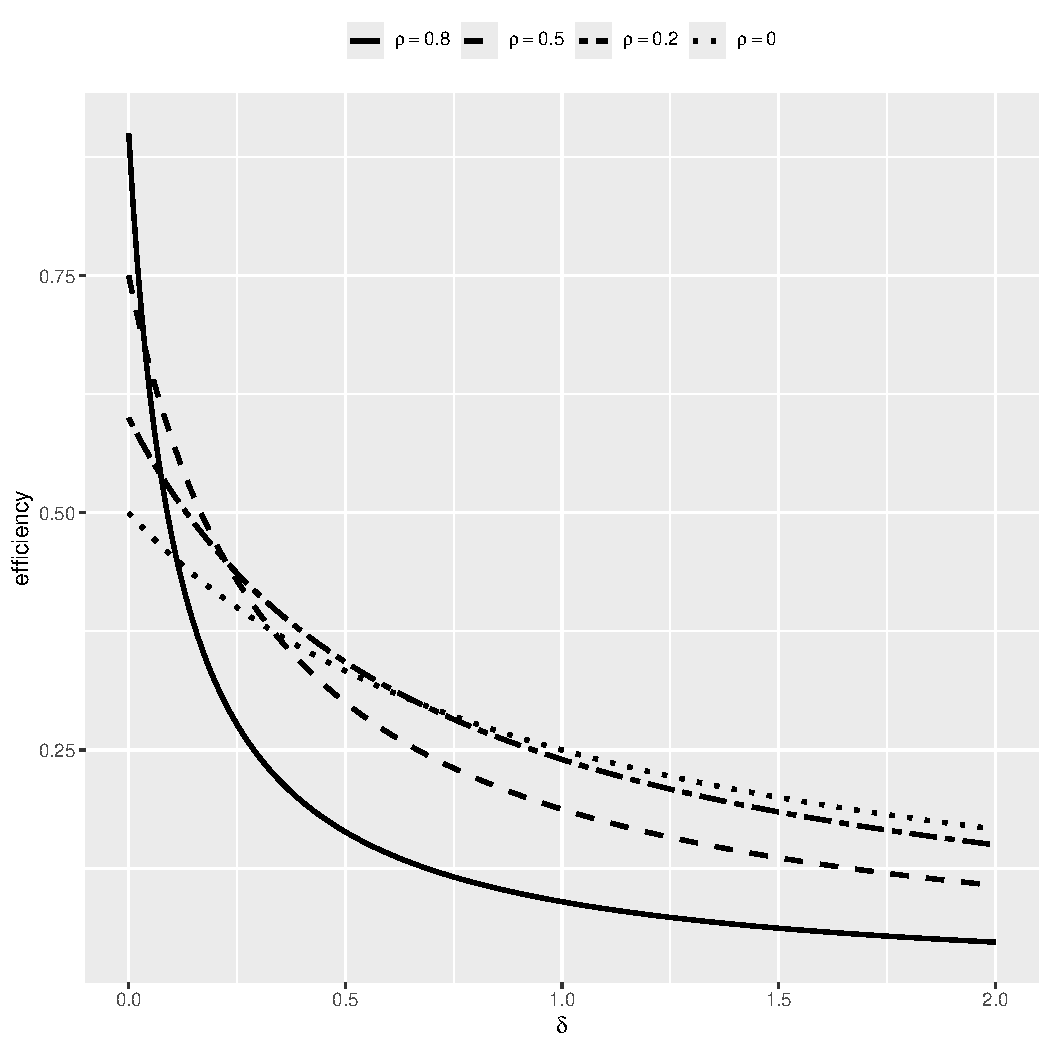
\includegraphics[width=\maxwidth]{figure/unnamed-chunk-7-1} 
\end{knitrout}

\newpage

\item[\scalebox{2.0}{\twemoji{keycap: 2}}] \hspace{0.3cm} $n = 5$.

\begin{knitrout}
\definecolor{shadecolor}{rgb}{0.969, 0.969, 0.969}\color{fgcolor}\begin{kframe}
\begin{alltt}
\hldef{df2} \hlkwb{<-} \hlkwd{data.frame}\hldef{(delta,}
                  \hlkwc{efficiency1} \hldef{=} \hlkwd{e}\hldef{(}\hlkwc{delta} \hldef{= delta,} \hlkwc{rho} \hldef{=} \hlnum{0.8}\hldef{,} \hlkwc{n} \hldef{=} \hlnum{5}\hldef{),}
                  \hlkwc{efficiency2} \hldef{=} \hlkwd{e}\hldef{(}\hlkwc{delta} \hldef{= delta,} \hlkwc{rho} \hldef{=} \hlnum{0.5}\hldef{,} \hlkwc{n} \hldef{=} \hlnum{5}\hldef{),}
                  \hlkwc{efficiency3} \hldef{=} \hlkwd{e}\hldef{(}\hlkwc{delta} \hldef{= delta,} \hlkwc{rho} \hldef{=} \hlnum{0.2}\hldef{,} \hlkwc{n} \hldef{=} \hlnum{5}\hldef{),}
                  \hlkwc{efficiency4} \hldef{=} \hlkwd{e}\hldef{(}\hlkwc{delta} \hldef{= delta,} \hlkwc{rho} \hldef{=} \hlnum{0.0}\hldef{,} \hlkwc{n} \hldef{=} \hlnum{5}\hldef{))}
\end{alltt}
\end{kframe}
\end{knitrout}

\begin{knitrout}
\definecolor{shadecolor}{rgb}{0.969, 0.969, 0.969}\color{fgcolor}\begin{kframe}
\begin{alltt}
\hldef{df2_melted} \hlkwb{<-} \hldef{df2} \hlopt{%>%}
  \hlkwd{pivot_longer}\hldef{(}\hlkwc{cols} \hldef{=} \hlkwd{starts_with}\hldef{(}\hlsng{"efficiency"}\hldef{),}
               \hlkwc{names_to} \hldef{=} \hlsng{"efficiency_type"}\hldef{,}
               \hlkwc{values_to} \hldef{=} \hlsng{"efficiency"}\hldef{)}
\end{alltt}
\end{kframe}
\end{knitrout}

\begin{knitrout}
\definecolor{shadecolor}{rgb}{0.969, 0.969, 0.969}\color{fgcolor}\begin{kframe}
\begin{alltt}
\hldef{df2_melted} \hlopt{%>%}
  \hlkwd{ggplot}\hldef{(}\hlkwd{aes}\hldef{(}\hlkwc{x} \hldef{= delta,} \hlkwc{y} \hldef{= efficiency,} \hlkwc{linetype} \hldef{= efficiency_type))} \hlopt{+}
  \hlkwd{geom_line}\hldef{(}\hlkwc{linewidth} \hldef{=} \hlnum{1}\hldef{)} \hlopt{+}
  \hlkwd{scale_linetype_manual}\hldef{(}
    \hlkwc{values} \hldef{=} \hlkwd{c}\hldef{(}
      \hlsng{"efficiency1"} \hldef{=} \hlsng{"solid"}\hldef{,}
      \hlsng{"efficiency2"} \hldef{=} \hlsng{"dashed"}\hldef{,}
      \hlsng{"efficiency3"} \hldef{=} \hlsng{"twodash"}\hldef{,}
      \hlsng{"efficiency4"} \hldef{=} \hlsng{"dotted"}\hldef{),}
    \hlkwc{labels} \hldef{=} \hlkwd{expression}\hldef{(}
      \hldef{rho} \hlopt{==} \hlnum{0.8}\hldef{,}
      \hldef{rho} \hlopt{==} \hlnum{0.5}\hldef{,}
      \hldef{rho} \hlopt{==} \hlnum{0.2}\hldef{,}
      \hldef{rho} \hlopt{==} \hlnum{0.0}\hldef{))} \hlopt{+}
  \hlkwd{labs}\hldef{(}\hlkwc{x} \hldef{=} \hlkwd{expression}\hldef{(delta))} \hlopt{+}
  \hlkwd{theme}\hldef{(}\hlkwc{legend.position} \hldef{=} \hlsng{"top"}\hldef{,}
        \hlkwc{legend.title} \hldef{=} \hlkwd{element_blank}\hldef{())}
\end{alltt}
\end{kframe}
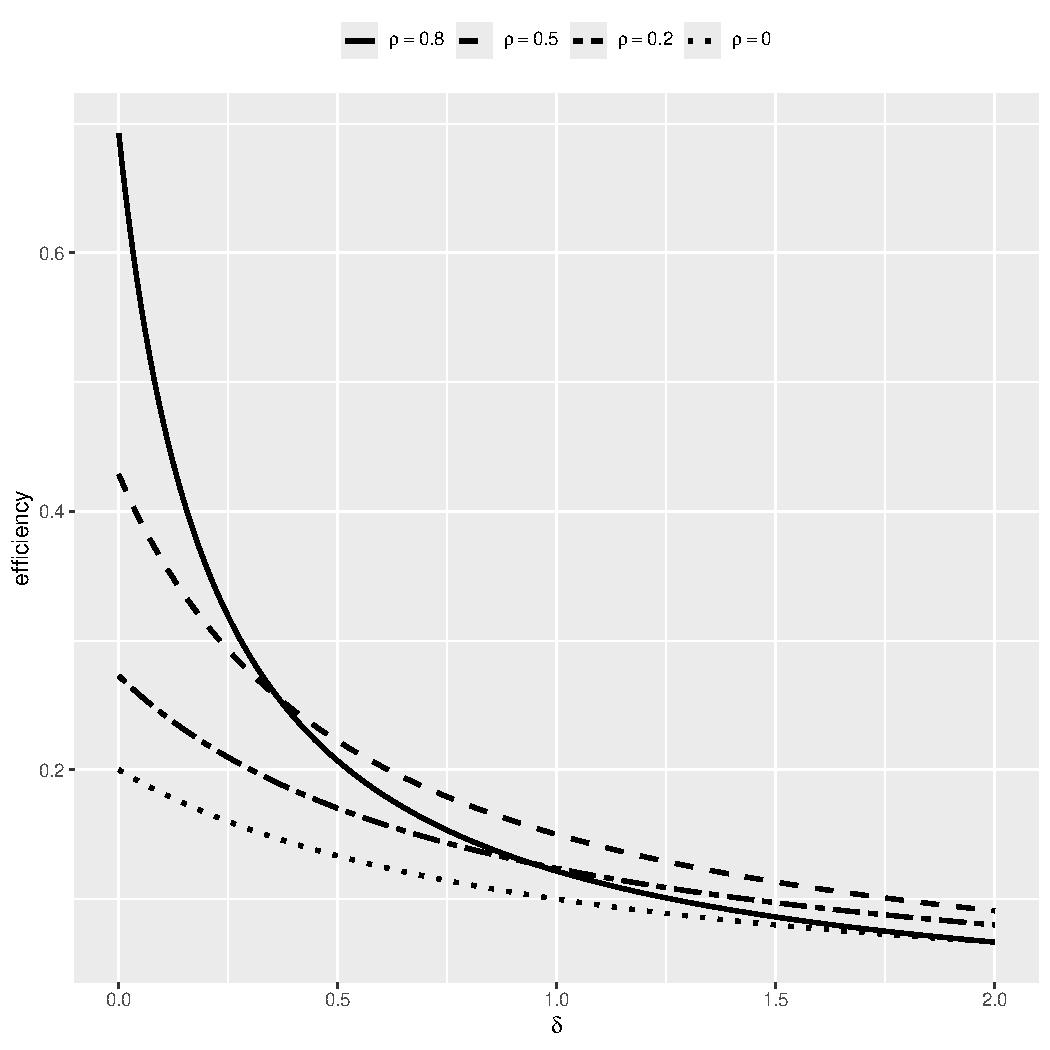
\includegraphics[width=\maxwidth]{figure/unnamed-chunk-10-1} 
\end{knitrout}

\newpage

\item[\scalebox{2.0}{\twemoji{keycap: 3}}] \hspace{0.3cm} $n = 10$.

\begin{knitrout}
\definecolor{shadecolor}{rgb}{0.969, 0.969, 0.969}\color{fgcolor}\begin{kframe}
\begin{alltt}
\hldef{df3} \hlkwb{<-} \hlkwd{data.frame}\hldef{(delta,}
                  \hlkwc{efficiency1} \hldef{=} \hlkwd{e}\hldef{(}\hlkwc{delta} \hldef{= delta,} \hlkwc{rho} \hldef{=} \hlnum{0.8}\hldef{,} \hlkwc{n} \hldef{=} \hlnum{10}\hldef{),}
                  \hlkwc{efficiency2} \hldef{=} \hlkwd{e}\hldef{(}\hlkwc{delta} \hldef{= delta,} \hlkwc{rho} \hldef{=} \hlnum{0.5}\hldef{,} \hlkwc{n} \hldef{=} \hlnum{10}\hldef{),}
                  \hlkwc{efficiency3} \hldef{=} \hlkwd{e}\hldef{(}\hlkwc{delta} \hldef{= delta,} \hlkwc{rho} \hldef{=} \hlnum{0.2}\hldef{,} \hlkwc{n} \hldef{=} \hlnum{10}\hldef{),}
                  \hlkwc{efficiency4} \hldef{=} \hlkwd{e}\hldef{(}\hlkwc{delta} \hldef{= delta,} \hlkwc{rho} \hldef{=} \hlnum{0.0}\hldef{,} \hlkwc{n} \hldef{=} \hlnum{10}\hldef{))}
\end{alltt}
\end{kframe}
\end{knitrout}

\begin{knitrout}
\definecolor{shadecolor}{rgb}{0.969, 0.969, 0.969}\color{fgcolor}\begin{kframe}
\begin{alltt}
\hldef{df3_melted} \hlkwb{<-} \hldef{df3} \hlopt{%>%}
  \hlkwd{pivot_longer}\hldef{(}\hlkwc{cols} \hldef{=} \hlkwd{starts_with}\hldef{(}\hlsng{"efficiency"}\hldef{),}
               \hlkwc{names_to} \hldef{=} \hlsng{"efficiency_type"}\hldef{,}
               \hlkwc{values_to} \hldef{=} \hlsng{"efficiency"}\hldef{)}
\end{alltt}
\end{kframe}
\end{knitrout}

\begin{knitrout}
\definecolor{shadecolor}{rgb}{0.969, 0.969, 0.969}\color{fgcolor}\begin{kframe}
\begin{alltt}
\hldef{df3_melted} \hlopt{%>%}
  \hlkwd{ggplot}\hldef{(}\hlkwd{aes}\hldef{(}\hlkwc{x} \hldef{= delta,} \hlkwc{y} \hldef{= efficiency,} \hlkwc{linetype} \hldef{= efficiency_type))} \hlopt{+}
  \hlkwd{geom_line}\hldef{(}\hlkwc{linewidth} \hldef{=} \hlnum{1}\hldef{)} \hlopt{+}
  \hlkwd{scale_linetype_manual}\hldef{(}
    \hlkwc{values} \hldef{=} \hlkwd{c}\hldef{(}
      \hlsng{"efficiency1"} \hldef{=} \hlsng{"solid"}\hldef{,}
      \hlsng{"efficiency2"} \hldef{=} \hlsng{"dashed"}\hldef{,}
      \hlsng{"efficiency3"} \hldef{=} \hlsng{"twodash"}\hldef{,}
      \hlsng{"efficiency4"} \hldef{=} \hlsng{"dotted"}\hldef{),}
    \hlkwc{labels} \hldef{=} \hlkwd{expression}\hldef{(}
      \hldef{rho} \hlopt{==} \hlnum{0.8}\hldef{,}
      \hldef{rho} \hlopt{==} \hlnum{0.5}\hldef{,}
      \hldef{rho} \hlopt{==} \hlnum{0.2}\hldef{,}
      \hldef{rho} \hlopt{==} \hlnum{0.0}\hldef{))} \hlopt{+}
  \hlkwd{labs}\hldef{(}\hlkwc{x} \hldef{=} \hlkwd{expression}\hldef{(delta))} \hlopt{+}
  \hlkwd{theme}\hldef{(}\hlkwc{legend.position} \hldef{=} \hlsng{"top"}\hldef{,}
        \hlkwc{legend.title} \hldef{=} \hlkwd{element_blank}\hldef{())}
\end{alltt}
\end{kframe}
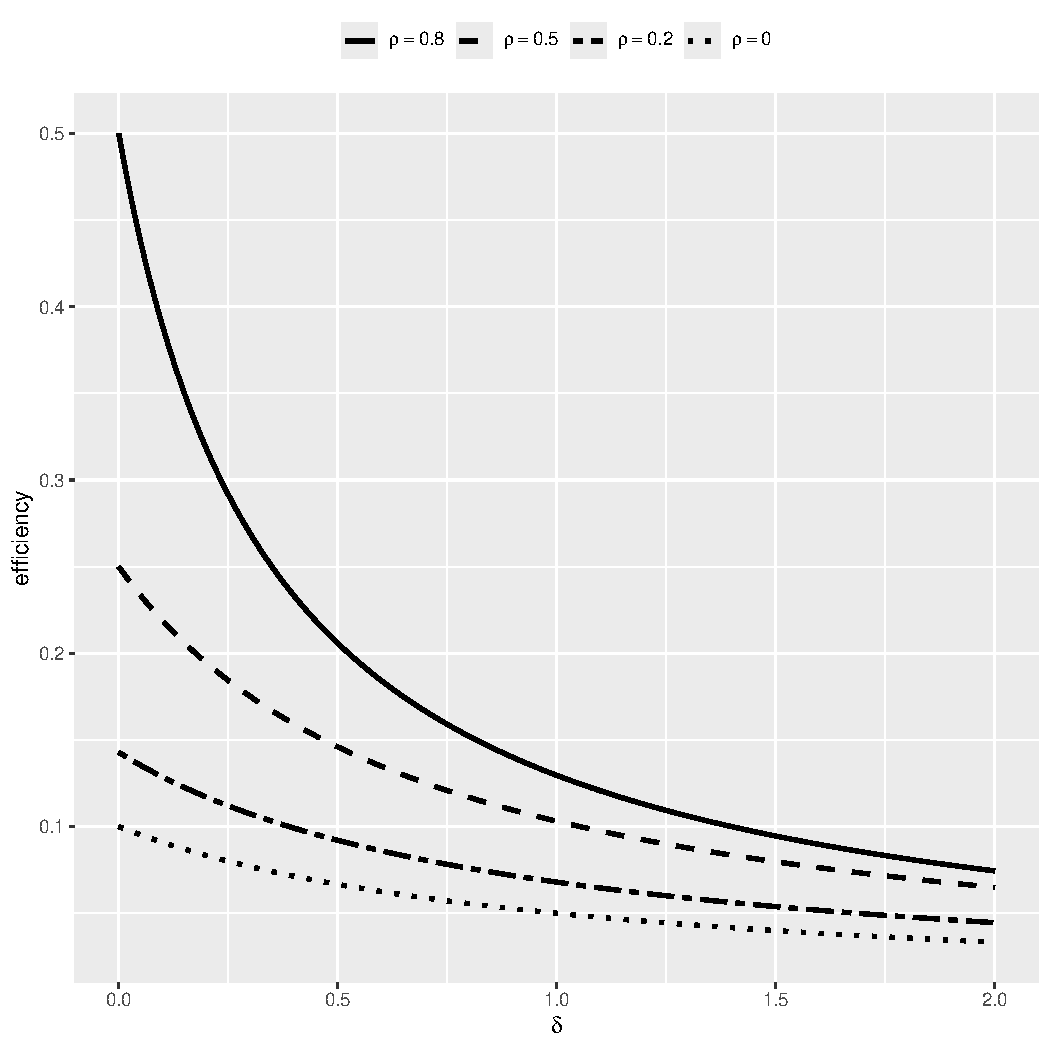
\includegraphics[width=\maxwidth]{figure/unnamed-chunk-13-1} 
\end{knitrout}


\smallpencil \hspace{0.1cm} {\fontsize{12}{20}\gloriahallelujahfont $e$ is a decreasing function of $\delta$. Except when $\delta$ is small and the common correlation $\rho$ is high, there is much to be gained by conducting longitudinal studies even when the number of repeated observations is as small as two.}

\end{itemize}



\end{document}
